\clearpage
\section{Simulation กับตัวควบคุม Linear Quadratic Regulator}
ในส่วนของการทดลองตัวควบคุมจะแบ่งออกเป็นสามส่วนคือ
\vspace{-10pt}
\begin{enumerate}[label=\arabic*), leftmargin=1.5cm]
	\setlength\itemsep{-0.25em}
    \item Altitude control
    \item Attitude control
    \item X Y Position control
\end{enumerate}
\vspace{-15pt}
\begin{figure}[!ht]
	\centering
	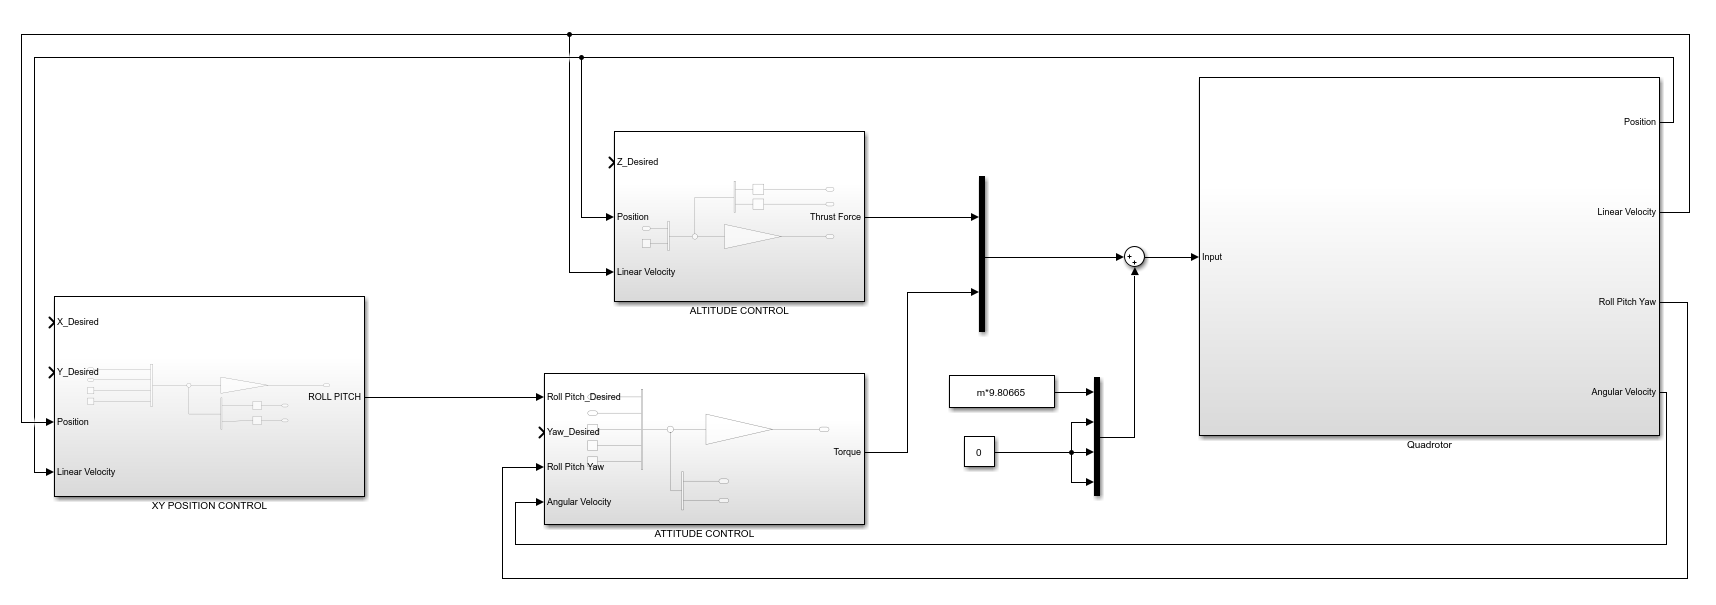
\includegraphics[width=0.8\textwidth]{images/simulink/lqr_all.png}
	\caption{แบบจำลองตัวควบคุม LQR ของ quadrotor ในโปรแกรม simulink}
\end{figure}

\subsection{Altitude control}
มี state และ input คือ
\begin{equation}
    {\vec{x}=\begin{bmatrix}
        z \\ v_z \\
    \end{bmatrix}, u = F_z}
\end{equation}

\paragraph*{การทดลองครั้งที่ 1}
กำหนดค่าน้ำหนักเมทริก $Q$ กับ $R$ ให้กับ Altitude control ดังนี้
\begin{equation}
    \begin{array}{c}
    {Q_{Altitude}=diag(\begin{bmatrix}
        1 & 1 \\
    \end{bmatrix})}\\[10pt]
    {R_{Altitude} = 1}\\[10pt]
    {K_{Altitude} = \begin{bmatrix}
        1 & 1.9885 \\
    \end{bmatrix}} \\
    \end{array}
\end{equation}

\begin{figure}[!ht]
	\centering
	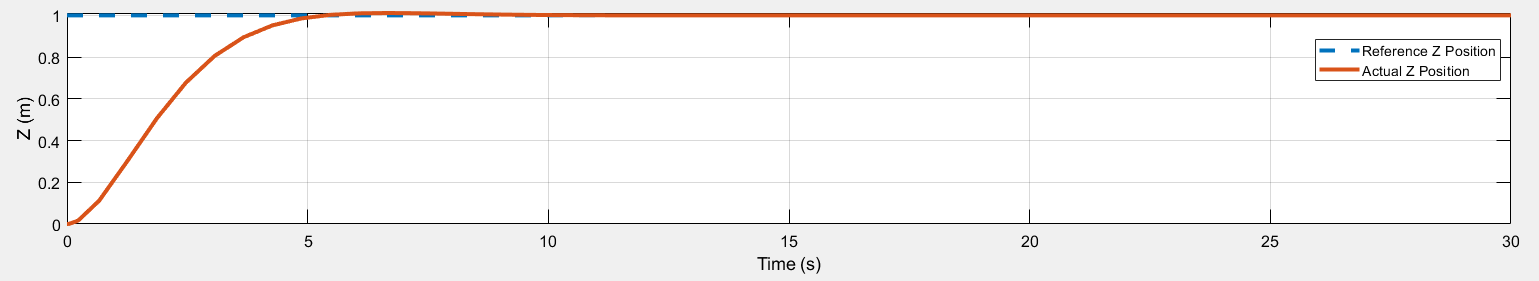
\includegraphics[width=0.8\textwidth]{images/simulink/altitude_control1.png}
	\caption{ผลการทดสอบ Altitude control ครั้งที่ 1}
\end{figure}

จากกราฟจะเห็นได้ว่าตำแหน่งตามแนวแกน Z ของ quadrotor สามารถลู่เข้าตำแหน่งที่ต้องการได้และใช้เวลาไปประมาณ 5 วินาที

\paragraph*{การทดลองครั้งที่ 2}
ต้องการให้ตำแหน่งตามแนวแกน Z ของ quadrotor ลู่เข้าสู่ตำแหน่งที่ต้องการได้เร็วขึ้น จึงได้กำหนดค่าน้ำหนักเมทริก
$Q$ กับ $R$ ขึ้นใหม่ดังนี้ 
\begin{equation}
    \begin{array}{c}
    {Q_{Altitude}=diag(\begin{bmatrix}
        10 & 1 \\
    \end{bmatrix})}\\[10pt]
    {R_{Altitude} = 1}\\[10pt]
    {K_{Altitude} = \begin{bmatrix}
        3.1623 & 3.2158 \\
    \end{bmatrix}} \\[10pt]
    \end{array}
\end{equation}

\begin{figure}[!ht]
	\centering
	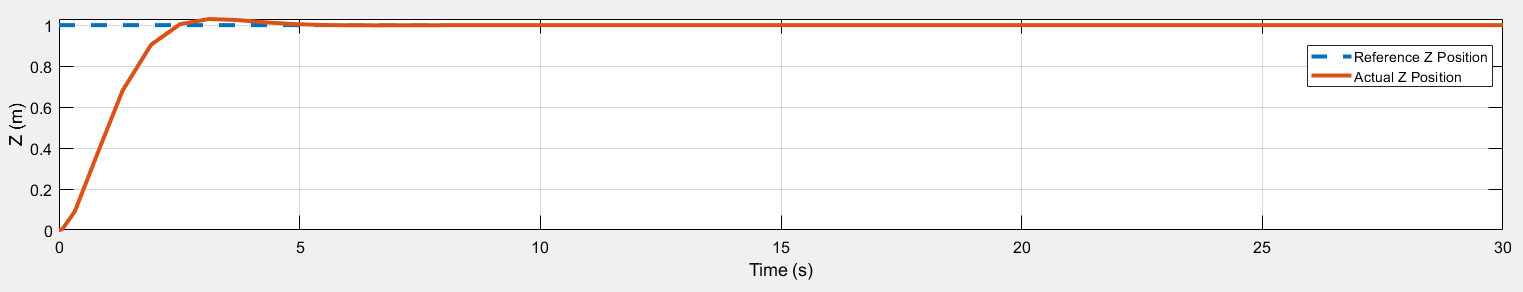
\includegraphics[width=0.8\textwidth]{images/simulink/altitude_control2.png}
	\caption{ผลการทดสอบ Altitude control ครั้งที่ 2}
\end{figure}
 
จากกราฟจะเห็นได้ว่าตำแหน่งตามแนวแกน Z ของ quadrotor สามารถลู่เข้า ณ ตำแหน่งที่ 1 เมตรเร็วขึ้น แต่มีการเกิด Overshoot ขึ้นเล็กน้อย

\subsection{Attitude control}
มี state และ input คือ
\begin{equation}
    {\vec{x}=\begin{bmatrix}
        \phi \\ \theta \\ \psi \\ p \\ q \\ r \\
    \end{bmatrix}, \vec{u} = \begin{bmatrix}
        \tau_x \\ \tau_y \\ \tau_z \\
    \end{bmatrix}}
\end{equation}

\paragraph*{การทดลองครั้งที่ 1}
กำหนดค่าน้ำหนักเมทริก $Q$ กับ $R$ ให้กับ Attitude control ดังนี้
\begin{equation}
    \begin{array}{c}
    {Q_{Altitude}=diag(\begin{bmatrix}
        1 & 1 & 1 & 1 & 1 & 1\\
    \end{bmatrix})}\\[10pt]
    {R_{Altitude} = diag(\begin{bmatrix}
        1 & 1 & 1\\
    \end{bmatrix})}\\[10pt]
    {K_{Altitude} = \begin{bmatrix}
        3.1623 & 3.2158 \\
    \end{bmatrix}} \\[10pt]
    \end{array}
\end{equation}